\documentclass{article}
\usepackage[utf8]{inputenc}

% 81 column comment
%01234567890123456789012345678901234567890123456789012345678901234567890123456789

% Reduce top margin, increase bottom margin
\usepackage[a4paper, top=3cm, bottom=4cm]{geometry} 
\usepackage{graphicx}		% images
\usepackage{hyperref}

\graphicspath{{images/}}

\title{Programming Assignment 2\\ CSC410 - Parallel Computing}
\author{Aaron G. Alphonsus}
\date{November 14, 2018}

\begin{document}
\maketitle

\section{Matrix-Vector Multiplication}

% Program description
A matrix-vector multiplication takes an input Matrix \textbf{A}, and a vector 
\textbf{B} and produces an output vector \textbf{C}. Each element of the output 
vector \textbf{C} is the dot product of one row of the input Matrix \textbf{A} 
and vector \textbf{B}, that is, \texttt{C[i] = $\sum_{j}$ A[i][j] $\cdot$ B[j]}.

\medskip
\noindent
This program contains the host program and CUDA kernel to multiply a square 
matrix with a vector.

\section{Performance Analysis}
In order to do the performance analysis, we used NVIDIA's profiling tool 
\texttt{nvprof}. This gave us the time taken by the kernel function as well as 
different CUDA API calls.

\medskip
\noindent
The Karp-Flatt metric provides a means to use empirical data to learn something 
about parallel overhead as well as the amount of inherently sequential 
computation in a parallel program. The basic idea is to collect data from 
several runs of the program with increasing numbers of processors.

\medskip
\noindent
\textbf{Definition:} Given a parallel computation showing a speedup $\psi(n, p)$
on $p$ processors, where $p > 1$, the experimentally determined serial fraction 
$f_e$ is defined to be: 
\[f_e = \frac{1/\psi(n, p) - 1/p}{1 - 1/p}\]
The speedup $\psi(n, p)$ is calculated as usual - the ratio between sequential 
execution time and parallel execution time.
\[\psi(n, p) = \frac{T(n, 1)}{T(n, p)}\]

\medskip
\noindent
With these formulas, we can benchmark our program. We assumed number of threads 
to be equal to $p$. We used a block size of 256 and increased number of blocks 
by 1 repeatedly. This is why the increase in $p$ is by 256 each time:
\begin{table}[ht]
\centering
\begin{tabular}{|c|c|c|c|c|c|c|c|c|}
\hline
$p$ & \textit{256}  & \textit{512}  & \textit{768}  & \textit{1024} 
    & \textit{1280} & \textit{1536} & \textit{1792} & \textit{2048} \\ \hline
$\psi(n, p)$ & $92.95$  & $175.93$ & $169.81$ & $224.40$ & $203.94$ & $239.84$ 
             & $224.87$ & $256.82$ \\ \hline
$f_e$ & $0.0069$  & $0.0037$ & $ 0.0046$ & $ 0.0035$ & $ 0.0041$ & $ 0.0035$ 
      & $ 0.0039$ & $ 0.0034$ \\ \hline
\end{tabular}
\end{table}

\medskip
\noindent
What we can see here is that the serial fraction is flattening out indicating 
that there is limited opportunity for more parallelism. We also notice that some
grid size / block size configurations are better than others in achieving 
speedup even though the total number of threads may be less. We hypothesize that
this is due to the design of the hardware.

\section{Algorithms and Libraries}
Our program follows the typical algorithm for a CUDA C program with a few 
differences:
\begin{enumerate}
    \item Declare and allocate host and device memory (we allocated unified 
    memory for the vectors).
    
    \item Initialize vectors on the host. For a quick and easy check of our 
    calculations, we initialized each row of \textbf{A} from \texttt{1} to
    \texttt{n} and the vector \textbf{B} from
    \texttt{1} to \texttt{n}. This means that each position in \textbf{C} is the
    sum of squares from \texttt{1} to \texttt{n} is given by the formula:
    \[ \frac{n (n + 1) (2n + 1)}{6} \]
    
    \item Transfer vectors from the host to the device. (This is a usual step i
    CUDA programs but since we declared unified memory, we did not have do
    this).
    
    \item Execute the matrix-vector multiplication kernel. We went with 
    coarse-grained parallelism with each thread multiplying a row of matrix 
    \textbf{A} with the vector \textbf{B}. The dot product summation was done 
    serially. 
    
    \item Transfer results from device to host (Not required since we used 
    unified memory).
    
    \item Free the unified memory.
\end{enumerate}

\medskip
\noindent
Libraries used:
\begin{itemize}
	\item The CUDA platform and API
    \item \texttt{<stdio.h>}
\end{itemize}

\section{Functions and Program Structure}
The program has 2 functions:
\begin{itemize}
    \item \texttt{main}
    \item \texttt{matvecMul}
\end{itemize}

\subsection{\texttt{main}}
Arguments: none

\medskip
\noindent
Returns: \texttt{0} indicating normal termination.

\medskip
\noindent
Description: 
\begin{itemize}
    \item Declares vectors and allocates unified memory to them.

    \item Initializes the vector \textbf{B} and each row of the matrix 
    \textbf{A} with numbers from \texttt{1} to \texttt{n}.

    \item Calls the CUDA kernel after defining grid and block sizes to execute 
    the multiplication in parallel.
    
    \item Prints out resultant vector \textbf{C}.
\end{itemize}

\subsection{\texttt{matvecMul}}
Arguments: 
    \begin{itemize}
	    \item \texttt{double *A}: Square matrix \textbf{A} of dimension 
	    \texttt{n * n}.
	    
	    \item \texttt{double *B}: Column vector \textbf{B} of length \texttt{n}.
	    
	    \item \texttt{double *C}: Result of matrix-vector multiplication, row 
	    vector \textbf{C} of length \texttt{n}.
	    
	    \item \texttt{int n}: Dimension variable for the matrix and vector (set 
	    to be 8192)
    \end{itemize}
Returns: void

\medskip
\noindent
Description:
\begin{itemize}
    \item CUDA kernel code that executes the matrix-vector multiplication on the
    GPU.
    
    \item Coarse-grained parallelism: threads run in parallel for each row of 
    the matrix
    \textbf{A} but execute the dot-product multiplication serially.
\end{itemize}

\section{Compilation and Usage}
Compilation: \texttt{nvcc -o prog2 prog2.cu} OR \texttt{make} 

\noindent
Usage: \texttt{./prog2}

\medskip
\noindent
The program can be compiled using the command \texttt{make}. To get rid of the 
executable in the folder, run the command \texttt{make clean}.

\medskip
\noindent
The program multiplies an \texttt{n x n} matrix with a vector of length 
\texttt{n}. The vector and each row of the matrix is filled with numbers from 
\texttt{1} to \texttt{n}. The resulting vector is the sum of squares from
\texttt{1} to \texttt{n} in each position. \texttt{n} is initialized as 
\texttt{8192}.

\section{Testing and Verification}
For verification as we built the program, we used small values of \texttt{n} 
and printed out all three vectors. The answers of the matrix multiplication were
verified using Maple. An example can be seen in figure \ref{fig:testing}.

\begin{figure}[ht]
	\centering
    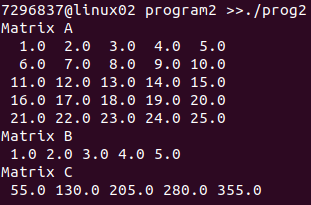
\includegraphics[width=0.25\textwidth]{5x5.png} \\
    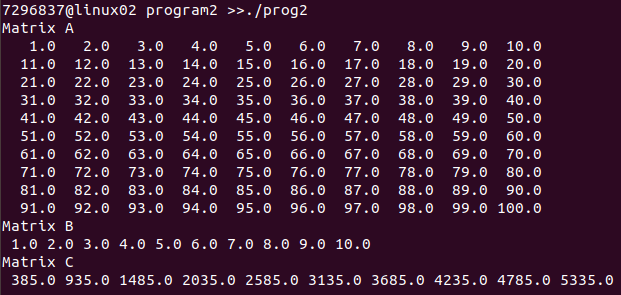
\includegraphics[width=0.55\textwidth]{10x10.png}
    \caption{Comparison of the static and dynamic schedulers}
    \label{fig:testing}
\end{figure}

\medskip
\noindent
Once we had a correct solution, we wanted a quick way to test that the program 
continued to work as we increased the number of elements. To do this we 
initialized the vector and each row of the matrix with numbers from \texttt{1} 
to \texttt{n}. We did this so that we would have a closed form solution for the 
resulting vector (sum of squares).

\noindent
We then calculate the sum of squares, compare it with each element in our 
resultant matrix, count the mismatches, and print the count and the sum of 
squares to the screen. The resultant matrix is also printed to the screen along 
with the grid size and block size for verification.

\section{Files Submitted}
\begin{itemize}
    \item \texttt{prog2.pdf}
    \item \texttt{makefile}
    \item \texttt{prog2.cu}
    \item \texttt{latex/}
\end{itemize}


\end{document}